\documentclass[12pt, notitlepage]{article}
\usepackage[utf8]{inputenc}
\usepackage{graphicx}
\graphicspath{ {images/} }

\usepackage[english]{babel}
\usepackage[nottoc]{tocbibind}

\usepackage{hyperref}
\usepackage[left=3cm,right=3cm,top=2cm,bottom=2cm]{geometry}

\usepackage{bbm}

\usepackage{amsmath}
\usepackage{amsthm}
\usepackage{amsfonts}
\usepackage{amssymb}
\newtheorem{thm}{Theorem}[section]
\newtheorem{lem}[thm]{Lemma}
\newtheorem{prop}[thm]{Proposition}
\newtheorem{cor}[thm]{Corollary}
\newtheorem{conj}[thm]{Conjecture}
\newtheorem{exmp}[thm]{Example}

\usepackage{mathtools}
\usepackage{tikz-cd}

\usepackage{xcolor}

\theoremstyle{definition}
\newtheorem{defn}{Definition}[section]

\title{Notes on Homotopy Theory}
\author{Sayantan Khan}
\date{July 2017}

\usepackage{gentium}

\newcommand{\cat}[1]{\mathrm{#1}}
\newcommand{\id}{\mathrm{id}}

\begin{document}
\maketitle

\tableofcontents

\newpage

\section{Categorical preliminaries}
In this section, we'll define the categories we'll be dealing with in
the rest of the notes.  We'll also define some categorical
constructions: in particular the \emph{pushout} and the
\emph{pullback}.

\subsection{Some important categories}
\begin{description}
\item[$\cat{SET}$:] This is the category of sets, where the objects
  are sets, and the morphisms between objects are set maps.
\item[$\cat{TOP}$:] This is the category of topological spaces, where
  the objects are topological spaces, and the maps are continuous maps
  between topological spaces.
\item[$\cat{hTOP}$:] This is the category with the objects being
  topological spaces, but the maps are homotopy classes of continuous
  maps, rather than being continuous maps themselves.
\item[$\cat{TOP^0}$:] This is the category of pointed spaces, i.e. the
  objects are tuples of spaces and a basepoint in them, and morphisms
  are continuous maps that take basepoints to basepoints.
\item[$\cat{hTOP^0}$:] This is the homotopy category of pointed
  spaces, i.e.  the objects are the same as in $\cat{TOP^0}$, but the
  maps are homotopy classes of maps between pointed spaces.
\item[$\cat{TOP(2)}$:] This is the category of pairs of spaces. The
  objects here are $(X,A)$, where $A \subset X$, and a morphism from
  $(X, A)$ to $(Y, B)$ is a continuous map $f: X \to Y$ such that
  $f(A) \subset B$.
\item[$W(X,Y)$:] Here, $X$ and $Y$ are two topological spaces. The
  objects of $W(X,Y)$ are the continuous maps between $X$ and $Y$, and
  the morphisms are homotopies between maps.
\item[$\cat{TOP}_B$:] Given a fixed topological space $B$, an object
  in the category $\cat{TOP}_B$ is a topological space $X$ along with
  a map $f: X \to B$.  Given two objects $(X, f : X \to B)$ and
  $(Y, g : Y \to B)$, a morphism from the former to the latter is a
  continuous map $h$ from $X$ to $Y$ such that the following diagram
  commutes.
    \[
    \begin{tikzcd}
    X \arrow{r}{f} \arrow[swap]{dr}{h} & B  \\
    & Y \arrow{u}{g}
    \end{tikzcd}
    \]
    This is the \emph{category of spaces over $B$}.
  \item[$\cat{hTOP}_B$:] This is the homotopy category of $\cat{TOP}_B$, where the
    objects are the same, but the maps are quotiented out by homotopies.
  \item[$\cat{TOP}^A$:] Given a fixed topological space $A$, an object in the
    category $\cat{TOP}^A$ is a space $X$ along with a map $f: A \to X$. Given
    two objects $(X, f: A \to X)$ and $(Y, g: A \to Y)$, a morphism between these
    objects is a map $h: X \to Y$ such that the following diagram commutes.
    \[
    \begin{tikzcd}
    A \arrow{r}{f} \arrow[swap]{d}{g} & X \ar{dl}{h}  \\
    Y & \\
    \end{tikzcd}
    \]
    This is the \emph{category of spaces under $A$}.
  \item[$\cat{hTOP}^A$:] This is the homotopy category of $\cat{TOP}^A$,
    described in a manner similar to $\cat{hTOP}_B$.
\end{description}

\subsection{Categorical constructions}
\subsubsection{Product}

\begin{defn}
  Given two objects $A$ and $B$ in a category $\mathcal{C}$, their
  product is an object $A \times B$ along with maps
  $\pi_1 : A \times B \to A$ and $\pi_2 : A \times B \to B$ such that
  for any object $F$ with maps $f_1 : F \to A$ and $f_2: F \to B$,
  there exists a unique map from $F$ to $A \times B$ making the
  following diagram commute.
\[
\begin{tikzcd}
&      F \arrow[swap]{dl}{f_1} \arrow{dr}{f_2} \arrow[dashed]{d}{\exists !}     & \\
A & A \times B \arrow{l}{\pi_1} \arrow[swap]{r}{\pi_2}  & B \\
\end{tikzcd}
\]    
\end{defn}

Products may not exist in all categories, but when they do, they are
unique.  They exist in $\cat{SET}$ and $\cat{TOP}$, are the usual
cartesian product.

\subsubsection{Coproduct}

\begin{defn}
  In a category $\mathcal{C}$, the coproduct of objects $A$ and $B$ is
  the object $A \coprod B$ along with maps $i_1: A \to A \coprod B$
  and $i_2: B \to A \coprod B$ such that for any pair of maps
  $g_1 : A \to G$ and $g_2: B \to G$, there exists a unique
  factorization via $A \coprod B$.
    \[
    \begin{tikzcd}
    A \ar{r}{i_1} \ar[swap]{dr}{g_1} & A \coprod B \ar[dashed]{d}{\exists !} & B \ar[swap]{l}{i_2} \ar{dl}{g_2} \\
    & G & \\
    \end{tikzcd}
    \]
\end{defn}

Coproducts exists in $\cat{SET}$ and $\cat{TOP}$ and are the disjoint
union in these two categories. In $\cat{TOP^0}$, the coproduct is the
wedge sum along the basepoint.

\subsubsection{Pullback}

\begin{defn}
  In a category $\mathcal{C}$, given two maps $f : X \to B$ and $g: Y \to B$,
  the pullback of $f$ and $g$ is the following diagram
    \[
    \begin{tikzcd}
    W \ar{r}{F} \ar[swap]{d}{G} & Y \ar{d}{g} \\
    X \ar[swap]{r}{f} & B \\
    \end{tikzcd}
    \]
    along with the universal property that for any $V$ with maps $F_V$ and
    $G_V$ to $X$ and $Y$, $F_V$ and $G_V$ factor uniquely through $W$.
    \[
    \begin{tikzcd}
    V \ar[bend left]{drr}{F_V} \ar[bend right, swap]{ddr}{G_V} \ar[dashed]{dr}{\exists !} & & \\
    & W \ar{r}{F} \ar[swap]{d}{G} & Y \ar{d}{g} \\
    &  X \ar[swap]{r}{f} & B \\
    \end{tikzcd}
    \]
\end{defn}
In $\cat{TOP}$, the pullback exists, and is given by the following
subspace.
\[
W = \{ (x,y) \in X \times Y\ |\ f(x) = g(y) \}
\]
Alternatively, a pullback can be shown to be the product in the
category $\cat{TOP}_B$.

\subsubsection{Pushout}

\begin{defn}
  A pushout is the dual notion to a pullback. Given a category $\mathcal{C}$, and maps
  $f: A \to X$ and $g: A \to Y$, the pushout of $f$ and $g$ is the following diagram.
    \[
    \begin{tikzcd}
    A \ar{r}{f} \ar[swap]{d}{g} & X \ar{d}{G} \\
    Y \ar[swap]{r}{F} & W \\
    \end{tikzcd}
    \]
    $W$ must also satisfy the following universal property.
    \[
    \begin{tikzcd}
    A \ar{r}{f} \ar[swap]{d}{g} & X \ar{d}{G} \ar[bend left]{ddr}{G_V} & \\
    Y \ar[swap]{r}{F} \ar[swap, bend right]{drr}{F_V} & W \ar[dashed]{dr}{\exists !} & \\
    & & V \\
    \end{tikzcd}
    \]
\end{defn}
In $\cat{TOP}$, the pushout $W$ is the following space.
\[
W = \frac{\left(X \coprod Y\right)}{f(a) \sim g(a)}
\]
Alternatively, a pushout can be seen as a coproduct in the category $\cat{TOP}^A$.


\section{Homotopical Constructions}
In this section, we'll cover the construction of the essential groups
and spaces in homotopy theory: the homotopy groupoid, mapping
cylinder, cones, suspensions, and loop spaces.

\subsection{Homotopy groupoid}
\begin{defn}
  Let $X$ and $Y$ be topological spaces. The category $\Pi(X,Y)$ has
  its objects as maps from $X$ to $Y$, and its morphisms are
  homotopies between maps quotiented by the following relation. Two
  homotopies between maps $f$ and $g$, $\mathcal{P}$ and $\mathcal{Q}$
  are the same morphism if there is a homotopy $\mathcal{M}$ from
  $\mathcal{P}$ to $\mathcal{Q}$ relative to \footnote{A homotopy
    relative to a subspace is a homotopy that is constant on that
    subspace.} $X \times \partial I$.
\end{defn}
The quotienting gives the collection of morphisms a groupoid
structure. In particular, associativity only works out because of the
quotienting. The fundamental groupoid is a special case of the
homotopy groupoid $\Pi(X,Y)$, when $X$ is just a point. Similarly, we
can describe the pointed version of the homotopy groupoid, which we
denote by $\Pi^0(X,Y)$ for pointed spaces $X$ and $Y$.

\subsection{Mapping cylinder}
\begin{defn}
  Given a map $f: X \to Y$, the mapping cylinder $Z(f)$ is constructed
  via the following pushout.
    \[
    \begin{tikzcd}
    X \ar{r}{f} \ar[swap]{d}{i_1^X} & Y \ar{d}{J} \\
    X \times I \ar[swap]{r}{a} & Z(f) \\
    \end{tikzcd}
    \]
\end{defn}
Topologically, the mapping cylinder is the disjoint union of
$X \times I$ and $Y$ quotiented with the relation $(x, 1) \sim f(x)$.
\begin{figure}[h]
    \centering
    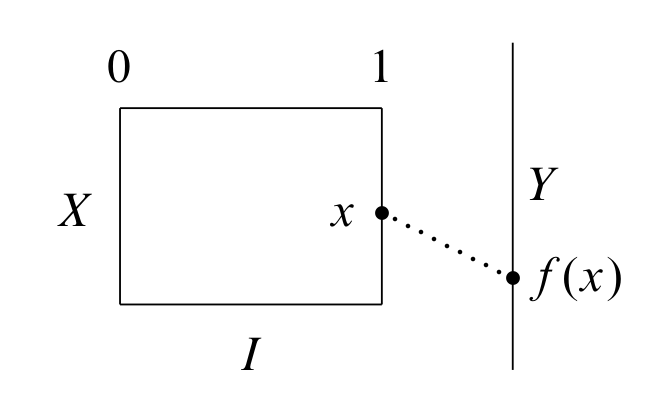
\includegraphics[scale=0.25]{mapping_cylinder.png}
    \caption{The mapping cylinder ({\color{red}Temporary. Put citation.})}
\end{figure}

We construct some more maps.
\begin{align*}
q: Z(&f) \to Y \\
q(x,t) &:= f(x) \\
q(y) &:= y  
\end{align*}
\begin{align*}
j: X &\to Z(f) \\
j(x) &:= (x, 0)
\end{align*}
We now have the following relations.
\begin{align*}
qj &= f \\
qJ &= \id_{Y}
\end{align*}
We can also see the map $Jq$ is homotopic to $\id_{Z(f)}$ relative to
the $Y$ subspace.  This means $Z(f)$ is homotopy equivalent to $Y$ and
$q$ and $J$ are the homotopy equivalence.  Note that $j$ is a closed
embedding. We have thus decomposed $f$ into a closed embedding $j$,
and a homotopy equivalence $q$.

\subsection{Suspension}
\begin{defn}
    content...
\end{defn}


%\bibliography{references}
%\bibliographystyle{amsplain}

\end{document}
